\documentclass{article}
\usepackage[review]{acl}

\usepackage{amsmath}
\usepackage{graphicx}
\usepackage{caption}
\captionsetup{justification=centering}
\usepackage{booktabs}
\usepackage{multirow}
\usepackage{hyperref}
\usepackage{natbib}

\title{COMP550 Final Project Writeup}

\author{
  James Lynch \\
  \And
  Jessica Wang \\
  \And
  Tyler Forgione \\
}

\begin{document}

\maketitle

\begin{abstract}
    We tried to replicate results on question answering data from big biomedical models like BioGPT or BioBERT while using far less training data. We fine-tuned three models, GPT-2, BERT, and T5, on QA data and used retrieval augmented generation techniques to improve their performance.
\end{abstract}


\section{Introduction}

Large Language Models (LLMs) benefit from the fact that the number of parameters they have is well above millions. Some even reach billions of parameters. They also benefit from the amount of data they are able to use during pre-training. This makes the models competent at a wide range of tasks.

Typical LLMs, used by many globally, are extremely well established at question answering (QA). The amount of knowledge they have on a number of different subjects makes them capable of answering most questions, save for some extremely difficult PhD level ones.

The biomedical field is one of the more difficult ones for the average LLM because of the amount of data in the field as well as the interactions between different parts of it. For example, drugs interact with diseases which have symptoms which may be side effects of other drugs or other diseases altogether. The model must be able to, given a question, filter through this information and deliver a clear and concise answer. In this project, we use datasets sampled from medical QA tests like the USMLE \cite{jin2020disease}, a dataset pulled directly from medical exams. We also use MedMCQA \cite{pmlr-v174-pal22a}, another multiple-choice QA dataset pulled from exams. These datasets include the types of questions that would stump smaller or less expressive models.

The USMLE dataset includes questions about choosing the correct condition given a number of symptoms and a patient's information. MedMCQA contains more textbook information, including facts about treatments, drugs, pathologies, and more.

Larger LLMs are able to answer these questions well above chance level \cite{liévin2023largelanguagemodelsreason}, however smaller models, like BERT \cite{devlin2019bertpretrainingdeepbidirectional}, are still in the $30\%$ range on these 4 option questions.

We explore whether models trained explicitly on biomedical question-answer data can come close to outperforming large models that are trained on a massive amount of general data. We attempt to use techniques in order to improve training as well as inference with as little cost as possible.

\section{Related Work}

Numerous models have already attempted to train on large biomedical corpora such as PubMed. One such model, PubMedBERT is based on BERT and pretrained from scratch on unlabeled biomedical data, mostly PubMed papers and abstracts \cite{Gu_2021}. Other models have been focused on training on biomedical data as a whole, as opposed to just papers. These models also perform well on the datasets described in the previous section. BioGPT \cite{Luo_2022} was a response to BioBERT \cite{Lee_2019} which used GPT's generative abilities to improve performance.

All of these models are pre-trained from scratch on millions (or more) of passages from biomedical textbooks, papers, articles, and more. Thus, they are trained on multiple GPUs for longer than we could afford to wait. In order to improve training times, as well as accuracy, we decided to implement retrieval augmented generation (RAG) \cite{lewis2021retrievalaugmentedgenerationknowledgeintensivenlp}, a technique in which the model retrieves data based on the prompt which it can use as context for the given task. It is a related but different idea to in-context learning. With RAG, the models are injecting explicit data that they can use for inference, while with ICL, this data is implicit to the prompt.

The benefit of RAG is that the model need not train on all the data but can instead just pull valuable passages that it can use to come up with an answer. This has previously been done in the biomedical field, starting with MedRAG \cite{xiong2024benchmarkingretrievalaugmentedgenerationmedicine}, an RAG framework that has been shown to improve the accuracy of GPT3.5 on most tasks, including the QA we look at. It is important to note that both the dataset the contexts are pulled from, as well as the retriever, are important in improving the model's performance. For example, Wikipedia's general knowledge may not help in USMLE style questions where knowing how conditions manifest matters. In that case, case studies seen in PubMed may be better.

Further, research has shown that fine-tuning RAG-augmented models may improve their accuracy even further \cite{hassan2025optimizingmedicalquestionansweringsystems}.

\section{Methods}

\subsection{GPT}
The Generative Pre-Trained Transformer (GPT) is a decoder only deep learning model. The GPT architecture has become widely adopted within the field of machine learning for a broad range of tasks, largely driven by chat-bots including Open AI's Chat-GPT and Anthropic's Claude. However, historically GPT models have not been used for classification tasks as the architecture is designed for text generation. This project aims to test whether GPT-2 (88.2 million parameters), a much smaller and older model, can achieve good performance in answering multiple choice medical questions. We will compare the results of our fine tuned GPT-2 model to BIO-GPT \cite{Luo_2022}.

For the multiple choice questions the prompt included the question first and then the 4 answer options (A-D). Before the question, an heading was concatenated "\#\#\# Question: " and before each option a similar heading was used, "\#\#\# Option (A-D)" \cite{Neural}. This was intended to provide structure to the prompt and make it easier for the model to separate the question and each of the answer choices. This concatenated string prompt was then tokenized using the tokenizer used by GPT-2. 

The GPT-2 model we used has a linear output layer of size 4 to facilitate the selection of an answer choice from A-D. The 183 thousand question MED-MCQA training dataset was used for fine tuning the model. For fine tuning we utilized LoRA \cite{hu2021loralowrankadaptationlarge} with a rank of 8 to limit the computational cost of training the model. A learning rate of $10^{-4}$ was used.

To improve results we utilized RAG \cite{lewis2021retrievalaugmentedgenerationknowledgeintensivenlp} using a corpus of textbooks frequently used to study for the USMLE. Each entry in the corpus was cut to only keep the first 100 tokens. Then all stop words were removed. Then the lexically most similar passage in the corpus to the question was selected through the BM25 algorithm \cite{lewis2021retrievalaugmentedgenerationknowledgeintensivenlp}. The passage was then added to the beginning of the prompt followed by the question and the answer choices. Note, due to limited computational resources RAG was only used during testing and was not used when fine tuning the dataset.

\subsection{BERT}
BERT \cite{devlin2019bertpretrainingdeepbidirectional} is an encoder-only transformer. This project aims to compare this general-purpose model and BioBERT \cite{Lee_2019} which was pre-trained on biomedical data text.

For multiple-choice QA, each (question, answer) pair is encoded independently as
\begin{equation}
    \texttt{[CLS]}\ q\ \texttt{[SEP]}\ a_i\ \texttt{[SEP]}
\end{equation}
The classification token embedding is then passed through a linear head to produce a score per option, which are are normalised with softmax and trained via cross-entropy. To avoid the cost of full finetuning, we used LoRA \cite{hu2021loralowrankadaptationlarge} with a rank of 32, which drastically reduces trainable parameters while maintaining comparable performance. Hyperparameters (learning rate $=3\times10^{-4}$ and batch size $=8$) were selected via a one-epoch grid search using the MedMCQA validation accuracy. Using the combination with the highest validation accuracy, models were finetuned on a shuffled combination of MedMCQA and USMLE, all with four options.

In order to increase accuracy, we also trained RAG \cite{lewis2021retrievalaugmentedgenerationknowledgeintensivenlp} variants, so the model learns from both the QA patterns and from the retrived medical knowledge. For each training example, the top three passages retrieved by the FAISS index \cite{douze2025faisslibrary} were prepended to the question before tokenisation, producing inputs of the form:
\begin{equation}
    \texttt{[CLS]}\ c_1\ c_2\ c_3\ q\ \texttt{[SEP]}\ a_i\ \texttt{[SEP]}
\end{equation}
with a 512-token limit. The retrieval corpus consisted of two MedRAG corpora: the medical textbooks corpora and a 150k sample of the Wikipedia corpus. Because the raw Wikipedia corpus contains a large proportion of non-medical content, it was first filtered with common medical terms. All passages were then chunked into 100-word segments and indexed using BM25s \cite{lewis2021retrievalaugmentedgenerationknowledgeintensivenlp}. At query time, the question text is tokenised and the top-$k$ passages with the highest BM25 scores are returned. We used $k=3$.

The final model was tested on MedMCQA, USMLE and GPQA.

\subsection{T5}

T5 is an encoder-decoder developed by Google. Its intruction-tuned version, Flan-T5 \cite{chung2022scalinginstructionfinetunedlanguagemodels} is what was used for this part of the project. The version used was flan-t5-xl, the largest available model. The reason for using this model was twofold: it would be most probable to get the best baseline accuracy due to its size, and it would be less likely to overfit (again due to its size). In this case, overfitting meant collapsing to selecting the same answer on multiple choice questions.

Further, this part of the project used a FAISS \cite{douze2025faisslibrary} index of MedRAG's Wikipedia, textbooks, and StatPearl corpora. The textbooks and StatPearl corpora were quite small, so they were used in full, while only 150k Wikipedia samples were chosen at random. These were then chunked into 100-word passages and indexed using FAISS. All in all, this came out to only 2GB of data; far less than the entirety of MedRAG, which is over 100GB.

To save time and memory, the model was allowed to use the top 3 contexts scored by the MedCPT retriever \cite{Jin_2023}. Then, the model was trained on QA data with RAG. That is, the model was allowed to train by answering retrieval-augmented questions, as opposed to just training on the questions alone. The idea was to allow the model to learn patterns in the questions, as well as learn information from the contexts retrieved from the FAISS index.

Because T5-xl is an extra large model, we furthered our efforts to save memory. Thus, we used 4-bit quantization \cite{dettmers2023qloraefficientfinetuningquantized} and Low-Rank Adaptation (LoRA) \cite{hu2021loralowrankadaptationlarge}. The quantization technique decreases the precision of the floating points used from default (16-bit in this case) to 4-bit. This saves memory at the cost of some accuracy, but it has been shown that accuracy does not suffer as much as expected. The last of our efforts used LoRA, which only uses a small subset of trainable parameters. The idea is that the updated weights are typically of low rank, so instead of training the full model and only updating low-rank weights, we only train with the low-rank weights. This makes the model much easier to fit in memory and decreases training time substantially.

This fine-tuned model was then tested on MedMCQA, USMLE, and GPQA.

\section{Results}

\subsection{GPT}
The testing accuracy for the pre-fine-tuned model with and without RAG on the MedMCQA and USMLE datasets is in table \ref{tab:GPTmedmcqa_preft}. Similarly the testing accuracy for the model fine-tuned on the MedMCQA dataset is in table \ref{tab:GPTmedmcqa_postft}. The USMLE task is significantly harder for GPT than the MedMCQA task, with the model achieving approximately chance level accuracy on the USMLE task across all model configurations. Additionally, the model without fine tuning performs worse across all testing conditions. Interestingly RAG improved testing accuracy, even if only slightly, for the pre-fine-tuned model on both the MedMCQA and USMLE datasets. These results suggest that the LoRA fine tuning methodology that we utilized was flawed, but the RAG methodology offered slight improvements in performance.

\begin{table}[h]
    \centering
    \begin{tabular}{lcc}
        \hline
        \textbf{Method} & \textbf{MedMCQA} & \textbf{USMLE} \\
        \hline
        Pre-FT Baseline & 0.3166            & 0.2670          \\
        Pre-FT RAG      & 0.3169            & 0.2767          \\
        \hline
    \end{tabular}
    \caption{GPT accuracy on test datasets before fine-tuning.}
    \label{tab:GPTmedmcqa_preft}
\end{table}

\begin{table}[h]
    \centering
    \begin{tabular}{lcc}
        \hline
        \textbf{Method}  & \textbf{MedMCQA} & \textbf{USMLE} \\
        \hline
        Post-FT Baseline & 0.2596           & 0.2420          \\
        Post-FT RAG      & 0.2596            & 0.2420          \\
        \hline
    \end{tabular}
    \caption{GPT accuracy on test datasets after fine-tuning.}
    \label{tab:GPTmedmcqa_postft}
\end{table}

\subsection{BERT}

\subsection{T5}

The baseline accuracies for the T5 model are shown in table \ref{tab:medmcqa_preft}. Immediately, it is noticeable that USMLE is a harder dataset. This is due to the fact that instead of exam-like questions, they are more case studies. As mentioned in the introduction, these questions ask the student to correctly identify a condition based on some symptoms and patient factors.

\begin{table}[h]
    \centering
    \begin{tabular}{lcc}
        \hline
        \textbf{Method} & \textbf{MedMCQA} & \textbf{USMLE} \\
        \hline
        Pre-FT Baseline & 0.282            & 0.280          \\
        Pre-FT RAG      & 0.322            & 0.273          \\
        \hline
    \end{tabular}
    \caption{T5 accuracy on test datasets before fine-tuning.}
    \label{tab:medmcqa_preft}
\end{table}

The model was then fine-tuned on balanced split over all labels from both USMLE and MedMCQA. In total, the model was trained on $22696$ examples, including the question \emph{and} contexts. See figure \ref{fig:t5train} for the loss, computed every 300 steps. To make sure the model was not collapsing, we tracked the number of outputs of each label. These did not show any crazy results and will not be shown.

\begin{figure*}[t]
    \centering
    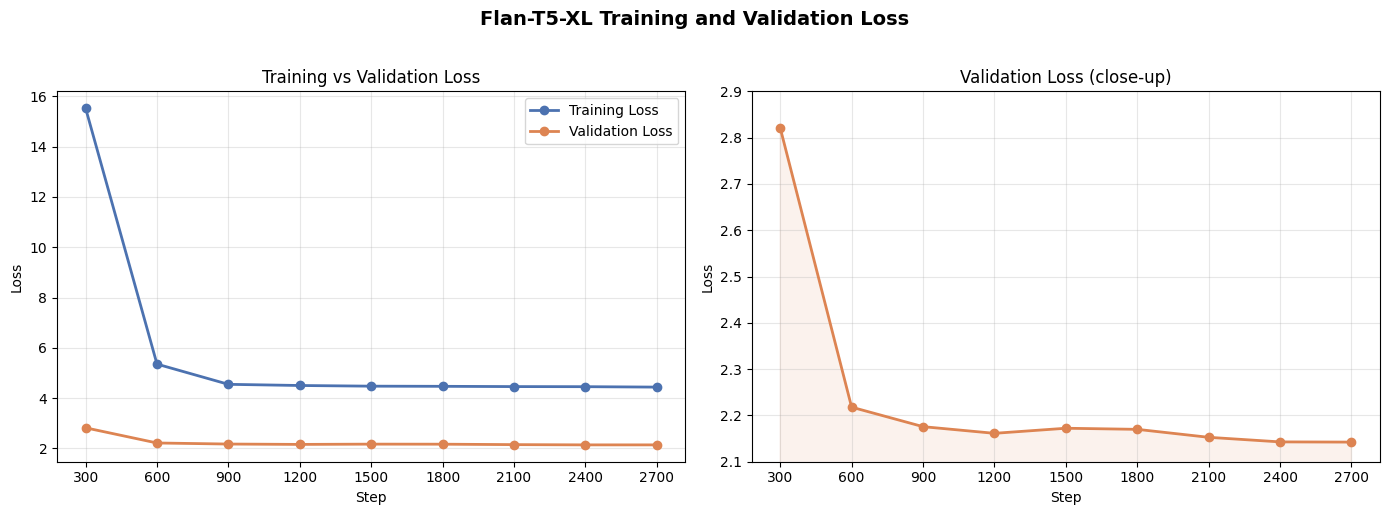
\includegraphics[width=\textwidth]{t5train.png}
    \caption{Training and validation loss visualization of flan-T5-xl}
    \label{fig:t5train}
\end{figure*}

Finally, the model was retested on the exact same test set as before fine-tuning. The results are shown in table \ref{tab:medmcqa_postft}.

\begin{table}[h]
    \centering
    \begin{tabular}{lcc}
        \hline
        \textbf{Method}  & \textbf{MedMCQA} & \textbf{USMLE} \\
        \hline
        Post-FT Baseline & 0.236            & 0.225          \\
        Post-FT RAG      & 0.239            & 0.227          \\
        \hline
    \end{tabular}
    \caption{T5 accuracy on test datasets after fine-tuning.}
    \label{tab:medmcqa_postft}
\end{table}

As a last resort, we checked whether the prompt was an issue. Thus, we tried including the options into the FAISS context retrieval and achieved the results in table \ref{tab:rag_results}.

\begin{table}[h]
    \centering
    \small
    \setlength{\tabcolsep}{4pt} % default is ~6pt
    \begin{tabular}{l c}
        \hline
        \textbf{Dataset}                 & \textbf{Accuracy} \\
        \hline
        USMLE (Post-FT RAG, q+options)   & 0.228             \\
        MedMCQA (Post-FT RAG, q+options) & 0.290             \\
        \hline
    \end{tabular}
    \caption{Test set accuracy for Post-FT + RAG (question + options)}
    \label{tab:rag_results}
\end{table}

\section{Discussion \& Conclusion}
In this report we investigated the performance of GPT, BERT, and T5 large language models on multiple choice medical questions from the MedMCQA and USMLE dataset. We found that none of the models achieved testingt accuracy above 32\% for MedMCQA and 28\% for USMLE. Considering chance level performance is 25\% our models are not able to reliably answer medical multiple choice questions. 

Our GPT model showed worse performance after fine-tuning with LoRA than the pre-fine-tuned model. However, the pre-fine-tuned model showed a slight improvement in performance when RAG was used across both the MedMCQA and USMLE datasets. Additionally, the GPT model had worse testing accuracy for the USMLE dataset then the MedMCQA dataset, suggesting it is a more difficult task. Overall, our GPT models were unsuccessful in exceeding the performance of BIO-GPT which has been found to have a 78.2\% accuracy on PubMedQA. Although, we did not test on PubMedQA directly our highest achieved accuracy for GPT was just under 32\% on the MedMCQA task suggesting significantly worse performance\cite{Luo_2022}.

Our T5 model had an accuracy increase of $4\%$ on the MedMCQA test set but actually dropped in accuracy on the USMLE dataset when only using RAG (no fine-tuning). This is likely due to the more reasoning-heavy nature of USMLE. However, after fine-tuning, the model performed worse on both datasets overall, dipping below chance. Originally, this was caused by a collapse in the model's selection of labels (e.g: always selecting C). After fixing this, the model still performs just as poorly.

The drop in performance could be due to overfitting, however the train and validation loss do not corroborate this. It would have been better to track accuracy on the training and validation set, but this would've increased training time too much.

After looking at the poor retrievals for certain questions, we opted to use the same evaluation, except for including the options into the FAISS retrieval. These results show a massive improvement on the fine-tuned model on MedMCQA and a small increase on USMLE for the same model. In all likelihood, the contexts were insufficient during training, as some questions are of the "which of the below are correct" sort. Thus, including the options would help. In the future, using better prompting and FAISS retrieval would be a focus.

\section{Statement of Contributions}

All preprocessing, training, and testing was done separately. James worked with GPT, Jessica worked with BERT, and Tyler worked with T5.

\bibliography{ref}

\end{document}